\documentclass[twocolumn,letterpaper,10pt]{article}
\usepackage{graphicx,amsmath}
\usepackage{epsf}
\usepackage[round]{natbib}
\usepackage{txfonts}
\usepackage{upgreek}
\usepackage{rotating}
\usepackage{epstopdf}
\usepackage{abstract}
\usepackage{hyperref}
\usepackage{geometry}
\geometry{margin = 0.75in}

\setlength{\bibsep}{0.0pt}

\def \um {$\mu m$}

\title{Monte Carlo Constraint of Luminosity Evolution and Redshift of Far-Infrared Galaxy Surveys}
\author{Noah Kurinsky and Anna Sajina\\*
  \small Tufts University\\*
  \small Department of Physics and Astronomy}
\date{\small \today}

\begin{document}
\twocolumn[
  \vspace{-0.5in}
  \maketitle
  \begin{onecolabstract}
    \centering
    To be written, updated form
  \end{onecolabstract}
  \vspace{1cm}
]

\section{Introduction}
In the field of observational astrophysics, a great deal of time is put into characterizing various properties of surveys of galactic populations both large and small. The vast majority of these efforts focus on an analysis specific to the survey, instrumentation, and source type being studied, and each requires new computer code and months of work to produce a publishable result. The necessity of such a time commitment makes maximizing the scientific yield of such analyses a top priority. Recent attempts have been made to characterize the properties of galaxy populations by using very general spectral features (e.g. spectral color) to fit complex evolutionary models \citep[e.g. redshift-luminosity evolution, as in ][]{marsden11}. A discussion of such methods, as well as their successes and failures, can also be found in the previous reference.

We extend the ideas presented in \citet{marsden11} from one spectral color to two; whereas they attempt to fit their model using the single 60-100 $\mu$m color, we instead employ a two color model, using three spectral bands, to create a two-dimensional diagnostic spectral color density plot of an observed population. We then employ a library of luminous and ultra-luminous infrared galaxy (LIRG and ULIRG) spectral energy distribution (SED) models to try to reproduce the observed trend, exploring the parameter space to constrain the redshift evolution of the far-infrared luminosity function. Using the luminosity function as a general prescription for number density and luminosity of galaxies at a given redshift, we can use the constrained parameters to simulate a high-redshift survey, given characteristics of the instrument performing the survey.

Our novel approach allows us to characterize the sample under examination as well as highlight the successes and failure of the SED template and the luminosity function form used by the fitting procedure. In addition, a large emphasis has been put on ensuring that the fitting program is highly generalizable; the models are stored externally to the main program in FITS format, and the luminosity function and various other procedures are highly modularized in the C++ code. Due to these features, the templates desired by the user can be specified at runtime, and the luminosity function can be easily modified. The program is not band or instrument specific, and the user can specify the exact survey characteristics (such as magnitude limits and statistical noise levels) to achieve the best fit possible. Such considerations allow us to address the need for reusable code, with the intent being that the analysis of data sets of this nature can be done much quicker, and result in a larger, richer science yield. In addition, we see high dependence of survey outcome on instrumental properties, and thus ability to tweak such characteristics has a large impact on the success or failure of fitting attempts.

The above is a very general description of the product we detail in this paper. We begin by discussing the assumptions made by the current form of the fitting procedure, such as luminosity functional form as well as the form of the redshift and model distributions. We then discuss the mathematical methods employed to randomize the simulation, perform the fitting, and generate the fitting statistic. We then present the results of testing the program with two far-infrared data samples of the GOODS-North field obtained by BLAST \citep{BLAST} and the Spitzer FLS field obtained by the HerMES survey \citep{HerMES}, using Herschel's SPIRE instrument \citep{Herschel,SPIRE}. These data sets measure identical bands, but differ in sensitivity, sample size, sky coverage, and other minor respects. We finally lay out the improvements that we plan to implement in the near future, and our eventual goals pertaining to public release and long-term usability for the project. 

\section{Simulating Galactic Populations}

To produce a simulated galaxy population suitable for comparison to an observed population (given the analyses described later in this paper), three flux densities corresponding to three distinct bands of observation need to be produced, in numbers which reduce statistical error to an experimentally acceptable level. The models employed must be able to reproduce characteristics of a wide range of galaxies, thus a set of models must be chosen that can generally describe any galaxy. In the far-infrared regime of the electromagnetic spectrum, the vast majority of radiation from galaxies is dust-reprocessed thermal radiation, and thus the emissions from these galaxies can be characterized by a blackbody, or more accurately, a modified blackbody (see Section \ref{sec:SED}). Choosing a model derived from physical formulae, as opposed to an empirical model, allows our eventual fits to speak more to the physical characteristics of the galaxy population, which in turn allows us to eventually infer star-formation rates as well as some other basic properties simply from the combination of temperature and luminosity.

Following the above reasoning, the first step in the simulation process is to generate a template of spectral energy distributions (SEDs) of the galaxies, from which flux densities can be pulled and to which parameter distributions can be ascribed. At first glance, it would seem as though such a library alone would be adequate for the simulation purposes, however observational surveys aren't perfect data products, and thus additional corrections must be made for factors such as statistical noise characteristic of the detector in use as well as the magnitude limit of the sample. In order to correct for these and other factors, it is necessary to adopt a luminosity function, with the added ability to randomly produce luminosities for sources in accordance with their likelihood as prescribed by the function. Additionally, a luminosity distance calculator is necessary, to convert luminosities into flux densities that can be used to normalize a given SED, such that noise can be added in a realistic manner to the template. The functional form of these and other components of the simulation, as well as details of their implementation, are described later in this section.

To be able to test the accuracy of the model against observation, a diagnostic needs to be chosen which can capture as many aspects of the sample as possible. Single fluxes have little meaning, as they vary with luminosity and distance, however, the trend over the entire simulated regime is luminosity independent, and provides a means by which to identify different sub-groups of similar sources. We choose to use the spectral color (defined as $S_\nu\propto\nu^\alpha$) to characterize each source, and produce a two-dimensional histogram of the entire population from these colors to describe the cumulative properties of the sample. The construction of this histogram and the method of comparison are described later in this section.

Even though the following sections describe specific implementations of the various aspects of the fitting program, it is important to note that many of these specific forms are only those adopted for our far-infrared fitting and modeling methods. The program has been designed and implemented to work with arbitrary models, and none of the specific details discussed below are actually present in the compiled executable, but are read in from files and are fully changeable. The luminosity function may, in the future, operate in a similar way; currently it is hard-coded. The overall design of the program is to strive for as few specific assumptions as possible. With this consideration in mind, we move on to discuss the specific assumptions made for the early version of this program.

\subsection{SED Library}\label{sec:SED}

In the previous version of this program, we employed a two-dimensional model comprised of modified blackbodies of various temperatures and radio strengths, without assigning them intrinsic luminosities. This served to model the very general properties of high-redshift, actively star forming galaxies, however more detailed models exist, and using such models enhances the robustness of our analysis. In this iteration of the program, we chose to adopt a library of SED templates from \citet{rieke09}, who construct a set of templates from a combination of local observations and radiative transfer arguments. These templates, seen in figure \ref{slib}, have associated intrinsic luminosities, due to their adaptation from real local galaxies, and range in far-infrared luminosity from $10^9 - 10^{13} L_{sun}$. A closer view of our specific region of interest, with the brightest and faintest SEDs at redshifts between $z\sim 0-5$, can be seen in figure \ref{mshift}.

These templates are mainly based on spectra obtained from a handful of local IRAS galaxies selected for having high star formation rates, which leads to a question of whether they remain valid models at high redshift. \citet{rieke09} discuss model validity up to redshifts around $z\sim2.5$, and conclude that their models can be considered fairly accurate for mid-infrared analyses, although they suggest that some boosting due to AGN should be added. It has also been suggested\footnote{by Professor Danilo Marchesini, Tufts University} that, due to the intrinsically larger nature of high-redshift galaxies, the intrinsic luminosities should also be evolved with redshift to a certain extent. As we will mention in the initial results (section \ref{example}), we do see a failure of models at high redshift to reproduce observation, which suggests that these models may need one of the suggested modifications. We are currently working on a much more robust template in parallel with this effort, which incorporates such color evolution with redshift.

The design of this program allows for consideration of model accuracy, and thus it might be best in future iterations to use a more robust library of models which has built in redshift evolution. We plan to re-adopt features for this program which allow for multiple models to be associated with the same intrinsic luminosity. There is a possibility that the user would specify in what proportion each model would be sampled in a given redshift regime, however it seems more likely that the program would add such considerations into its fitting efforts, and produce as output how successful various weightings are at reproducing observations. 

As noted in a previous version of this paper, and in \citet {wiklind03} (who employed modified blackbodies to constrain redshift far-infrared galaxies), the introduction of such considerations leads to a large amount of degeneracy, and for this iteration of the program our main concern was to implement the Monte Carlo fitting routine, thus we chose a simpler model template. Future versions will undoubtedly see a change, however as models are user specified, single luminosity models may be used and preferred depending on use cases.

\subsection{Luminosity Function}\label{sec:lf}

By far the most important component of the program, the luminosity function determines the number and luminosity of generated sources for a given redshift, which we modify by altering the manner in which the luminosity function evolves with redshift. This approach replaces the previous approach of using the luminosity function only to assign luminosities, and randomly selecting models and redshift distributions; now, the luminosity function determines all of these factors for us. For this version of the program we employ an IRAS-type double power-law luminosity function from \citet{negrello13}:
$$
\frac{dN}{dV dlogL}(L|L^*,\Phi^*,\alpha,\beta,z) = \Phi^*(z)*\left[{\left(\frac{L}{L^*(z)}\right)}^{\alpha}+\left(\frac{L}{L^*(z)}\right)^{\beta}\right]^{-1}
$$
where $\Phi^*$ and $L^*$ are evolved with redshift as described in \citet{Caputi07}:
$$
\Phi^*(z) = \Phi^*_0(1+z)^p \quad
L^*(z) = L^*_0(1+z)^q
$$
The default values for $\alpha$, $\beta$, $\Phi^*_0$, and $L^*_0$ for 350 $\mu$m were taken from \citet{negrello13}, and for this iteration are considered fixed values, as the luminosity function is well constrained at low redshift. The default values for p and q were taken from \citet{Caputi07} for redshift evolution out to $z\approx2$; the values we choose are those consistent with the low-redshift evolution from that paper. These values only serve as defaults, and can be altered via the interactive interface, as will be discussed below. For the current form of the program, we assume no evolution after redshift of $\sim2$, as is generally accepted due to analyses such as that presented in \citet{marsden11}. I will discuss how this translates to simulated source numbers in section \ref{generate}.

\subsection{Cosmology}

As we are simulating galactic populations spanning a large chunk of the observable universe, correct calculation of distance and volume as a function of redshift, as well as correct compensation for redshift effects, is vital to the accuracy of our effort. Specifically, we need to calculate luminosity distance, co-moving volume, and correctly apply K-corrections when calculating observed flux values. I describe the formulae we apply in this section, and discuss various approximations and special considerations. We adopt the cosmology from WMAP ($\Omega_{\Lambda}=0.728, \Omega_{M}=0.272, \Omega_k=0, H_0=70.4$) for our default values \citep{Komatsu11}.

\subsubsection{Luminosity Distance}
In order to convert luminosity and redshift into a flux, as well as determine the detectability of a source given the magnitude limit of a sample, the program needs to be able to compute luminosity distance. We decided to assume a flat universe (as evidenced above by $\Omega_k=0$), however all other cosmological parameters are left free, so that future users can adjust them as more accurate measurements are made. Our one assumption allows for the code to be faster and more efficient, and as it is commonly believed that our universe has no curvature, it should not affect the long-term value of this program.

Luminosity distance is computed by the standard formula:
$$
d_L(z)=\frac{(1+z)c}{H_0}\int\limits_0^z\frac{dz'}{\sqrt{(1+z')^3\Omega_M+\Omega_\Lambda}}
$$
We compute this using numerical integration in redshift steps of $z=0.001$ to maximize precision while allowing for real-time luminosity distance calculations. Future program versions will most likely see an interpolation based calculator, in order to increase performance, as every simulated flux currently requires a 1000 cycle integration operation.

\subsubsection{Comoving Volume}
In order to convert the luminosity function into a source number, we also need to compute the comoving volume for a given redshift bin. For the case of a flat universe, the co-moving volume per solid angle between $z_{min}$ and $z_{max}$ is:
$$
\frac{dV_C}{d\Omega}=\int_{z_{min}}^{z_{max}}\left(\frac{dV_c}{dz d\Omega}\right)dz\approx \left(\frac{dV_c}{dz d\Omega}\right)\Delta z
$$
for small $\Delta z$, where
$$
\frac{dV_c}{dzd\Omega}=\frac{c\,\left[d_L(z)\right]^2}{H_0 (1+z)^2 \sqrt{\Omega_M(1+z)^3+\Omega_{\Lambda}}}
$$
Here, all parameters are as defined for the luminosity distance calculation. Multiplication of $dV_C/d\Omega$ by the solid angle gives the total co-moving volume between the redshift bounds.
\subsubsection{K Corrections}

Due to observation in a fixed bandpass, and a red-shifting of the emission from the galaxy into the bandpass ($\nu_e=[1+z]\nu_o$), we need to correct for the varying size of the bandpass by multiplying the expected flux by an additional factor of (1+z):
$$
f_{\nu}(\nu_o)=\frac{(1+z)}{4\pi d_L^2}L_{\nu}(\nu_e)
$$
See \citet{Hogg02} for a more involved derivation and discussion.

\subsection{Observational Considerations}

In addition to simulating the theoretical SEDs produced by galaxies, a thorough fit of model to observation must take into account certain properties of the survey being analyzed. In the current version of the fitting program, random Gaussian noise representative of the average flux error is added independently to each simulated band after normalization by the luminosity function to simulate error due to unforeseen factors, mainly thermal noise in the case of our far-infrared bolometers. In addition, the magnitude limit is taken into consideration, and sources whose flux in any band falls below the detection threshold of the instrumentation are excluded from all analyses, although the number of ``undetectable'' sources produced by various parameter combinations is recorded, so that in the future it may be used somehow to improve the quality of the fit, or as an indication of the completeness of the survey.

Additionally, many surveys conducted to probe out to high-redshift are conducted in extremely dark areas of the sky, and are thus designed to minimize contamination by low-redshift sources. This leads to a dearth of low-redshift sources in the observation, which we account for in the simulation by setting the minimum redshift considered to a non-zero value. If not done, all simulations will be dominated by low redshift sources. This is user defined, however, and depending on the survey, different minimum redshifts may be employed to better reproduce the sample under consideration.

For the tests discussed in Section \ref{example}, the noise level was the experimentally found mean of the flux errors provided with the survey data, calculated separately for each band, and the flux limits were taken to be the minimum fluxes found in each band. We also assume a minimum redshift of $z\sim 0.1$, which is reasonable considering the depth of the field observed.

\subsection{Generating a Survey from SEDs and a Luminosity Function}\label{generate}

Our main goal is to attempt to recreate an observation with the basic assumptions that we have a prescriptive luminosity function, full set of SED templates, and correct characterization of the basic properties of our instrument. Imagining the simulation space as a two-dimensional space in luminosity and redshift, we break the space down into bins of $z$ versus $log(L_{fir})$. Assuming the intrinsic luminosities of the templates are equally spaced in log space (as they are in our case), they naturally break themselves into equal bins in the luminosity direction. We additionally break the redshift range into equal bins, with variable size specified by the user. The finite redshift bin sizes ensure that when we calculate source numbers, we get a large number of bins with non-zero integer source numbers.

For each bin, we calculate the number of sources to simulate using the formula
$$
N=\Omega \int\limits_{z_{min}}^{z_{max}}\int\limits_{L_{min}}^{L_{max}}\frac{dV_c}{dzd\Omega}(z)\frac{dN}{dV_c dlogL}(L,p,q,z) dLog(L)dz
$$
where the terms are as defined in the previous sections, and we assume that the parameters $\Phi^*_0,L^*_0,\alpha$ and $\beta$ are assumed to be fixed and determined at the start of run time. With our moderately sized bins, we approximate this as:
$$
N\approx\Omega \frac{dV_c}{dzd\Omega}(z_{avg})\frac{dN}{dV_c dlogL}(L_{avg},p,q,z_{avg}) \Delta Log(L) \Delta z
$$
We make this approximation for a few reasons. Firstly, we have no choice but to split the luminosity into bins, as be have binned SED models; they are already skewed towards the central luminosity, so it makes the most sense to find the prevalence of this luminosity and generate sources for luminosities surrounding it in equal proportions. 

We choose not to integrate in redshift due mainly to the computation expense; for every calculation of an infinitesimal co-moving volume element, we need to integrate to obtain luminosity distance for that redshift, and if we were to integrate over this element, we would be creating multiple large nested loops, increasing program runtime by orders of magnitude, without gaining appreciable precision. For these reasons, assuming the bins are small enough, we make this approximation without loss of generality and accuracy. Again, see \citet{negrello13} for an in depth discussion of this model.

With a two-dimensional integer populated space, we can begin to construct the simulated survey. For each redshift/luminosity bin, we perform the following sequence of steps:
\begin{enumerate}
\item Compute wavelength at which observed radiation would be emitted (according to $\lambda_{emit}=(1+z)^{-1}\lambda_{obs}$)
\item Extract the luminosity per unit wavelength at these wavelengths from the model with the luminosity associated with the given bin
\item Compute the k-corrected flux density at the given redshift
\item Simulate random instrumental noise for each flux based on the specified noise parameters
\item Check that the source is above the detection threshold of the simulated instrument in all three bands
\item If detected, add to overall source array
\end{enumerate}
This process is repeated the number of times indicated by the integer value in that redshift/luminosity bin, with the first step only completed once per redshift bin, and the second once per luminosity bin. 

In this manner, we are able to generate simulated surveys containing lists of three matched flux densities with standard errors and minimums matching those seen for the real survey; thus we isolate variation such that it exists only in source number, luminosity distribution, and redshift distribution, which we mainly control in this iteration through the manipulation of the luminosity function redshift evolution. 

\section{Fitting Methodology}

The simulated and observed galactic populations are compared on the basis of their spectral color distributions, as discussed in the introduction. In order to produce a statistic indicative of goodness of fit, a diagnostic plot which can characterize an entire population based on the spectral colors of the sources is needed, in order to produce a space within which the statistic can be run. For our fitting program, we employ a two-dimensional color histogram, of which each axis is a distinct spectral color. This is discussed in further detail in Section \ref{color_hist}. 

The fitting statistic used to compare observation and simulation is a $\chi^2$ statistic, computed as described in Section \ref{chisq}. The fitting is performed by systematically varying the parameters of the various distributions in an attempt to minimize the chi-square error. For the current version of the fitting program, this is a somewhat involved process, as the model parameters are currently fixed and must be altered by the user to find the parameter distributions which produce the best fit. This process will be described in more detail as an example of the fitting is described in Section \ref{example}.

\subsection{Two-Dimensional Spectral Color Histogram}\label{color_hist}

As with all fitting programs, one of the most important choices made in the design process is choosing the way in which to compile the data such that a fitting statistic can be run on it. Most programs tend towards one dimensional data representations, as these are much easier to handle. Due to the nature of our models and of sources in this particular regime of the electromagnetic spectrum, we decided on a two-dimensional color density metric. This data representation allows us to clearly identify multiple populations where present, as well as trends at both sides of the range of interest.

The diagnostic produced from the simulated data is a two dimensional histogram, with the 250\um/500\um\ color as the x axis and the 350\um/500\um\ color as the y axis. An example of this diagnostic for a real dataset can be seen in Figure \ref{fig:hist1}. There are in fact three unique color pairs that can be produced from fluxes in three distinct bands. This combination was chosen because the 500\um\ flux has a larger statistical error than the other two bands. This combination ensures that sources with largely erroneous 500\um\ fluxes will still exhibit the same general trend, but lie either lower or higher on the trend than they should be. This is not important for fitting purposes, as we add in simulated noise at comparable levels to that present in observation. It does allow for better identification of potential multiple populations by eye within a given sample and minimizes the visual noise obscuration such that overall trends are minimally disturbed.

\subsection{Chi-Square Testing}\label{chisq}

The major hurdle to working with higher dimensional metrics like this is the over abundance of zero values. Higher dimensional spaces tend to become largely empty as data sets become smaller, thus making the traditional goodness of fit methods harder to implement, as many behave poorly at small values and are undefined at 0. To help counteract this problem, we employ the binsize selection method outline in \citet{binsize}, where the ideal bin size for a sample of size $N$ with standard deviation $\sigma$ is: 
$$
\Delta \alpha=\frac{3.49\sigma}{\sqrt[3]{N}}$$
 This formula was experimentally found by \citet{binsize} to best balance the need to minimize whitespace and statistical error while maintaining as much resolution as possible.

The goodness of fit statistic we employ is the popular $\chi^2$ statistic, although a few minor alterations needed to be made to the general formula to obtain a statistic useful for our particular diagnostic, as well as to eliminate the "0" problem which plagues the traditional formula. To begin with, we assign the histogram bins standard Poisson errors \footnote{We currently employ the approximate form ($\sigma_i=\sqrt{N_i}$), but in subsequent versions will correct this to precise poisson error.}. Starting from the generalized chi-square formula:
$$
\chi^2=\sum\limits_{i=1}^n \frac{(O_i-E_i)^2}{\sigma_i^2}
$$
we get our fitting statistic by setting bin error to 
$$
\sigma_i=\sqrt{\sigma_{E_i}^2+\sigma_{O_i}^2}=\sqrt{E_i+O_i}
$$ 
The chi-square error is defined so long as one of the two diagnostics has a non-zero value. For zero values, the results are in agreement, so the formula is overridden and that particular bin is assigned a $\chi^2$ value of zero. The resulting piecewise $\chi^2$ formula then becomes:
$$
\chi^2=
\begin{cases}
\sum\limits_{i=1}^n \frac{(O_i-E_i)^2}{E_i+O_i}, & O_i > 0 \text{ or } E_i > 0 \\
0, & E_i=O_i=0
\end{cases}
$$
This approach ensures that for any given comparison, there exists a $\chi^2$ value, and gives more weight to areas of higher density, as they have lower comparable error to those bins with only a few sources.

\subsection{Markov Chain Monte Carlo Minimization}

The basic structure of Markov Chain Monte Carlo algorithms comprises a function which produces random deviations from an initial guess, and an algorithm which decides whether to accept these deviations as acceptable guesses. This is usually based upon the difference between the goodness of fit these parameters produce and the best goodness of fit obtained during the parameter space search; if the goodness of fit is better, it will automatically be accepted, otherwise the likelihood of acceptance will fall off exponentially. A detailed discussion of such algorithms as applied to cosmological parameter fitting can be found in \citet{dunkley05}.

Here, we employ the simplest form of such an algorithm, which is a type of ``Metropolis'' algorithm as it is defined in \citet{dunkley05}. Given initial parameter values obtained from the previous iteration, a random variate is produced according to a gaussian profile with a width specified by the user at run-time, which we refer to as the proposal distribution width; there are two such widths currently, one for p ($\sigma_p$) and one for q ($\sigma_q$), although the infrastructure exists for any number of parameters with associated widths. Thus if one were to track the random deviates of p, the probability of a given deviation would, in the large run limit, approach the distribution
$$
P(dp)=\frac{1}{\sqrt{2\pi\sigma_p^2}}\exp\left[{\frac{-(dp)^2}{2\sigma_p^2}}\right]
$$
This function is of course just a normalized Gaussian as one would expect; the same is true for q, assuming substitution of the correct width. Note here that the run number must be large enough for the deviates to approach this ideal curve; this highlights one of the reasons why we require large run numbers to produce appropriate statistical measures.

Acceptance of a guess generated according to the above mechanism is decided based on an analogy to the occupation probability of a classical gas; we consider the $\chi^2$ produced by the parameters as the ``energy'' of the system, and thus the probability of a system occupying such a state is given by
$$
P(E \, or \, \chi^2)\propto \exp\left[\frac{-E}{kT}\right] = \exp\left[\frac{-\chi^2}{T_s}\right]
$$
where of course $T_s$ is not strictly a temperature, as $\chi^2$ is a dimensionless quantity. We then accept or reject the guess by comparing the value of the above calculation to a random variate produced according to a flat distribution with values ranging from zero to one. The point here is just to show that, according to our algorithm, we can define a ``heat'' of our Monte Carlo, where a hotter run corresponds to greater probability of choosing $\chi^2$ values further from the best value and thus a more thorough sampling of the space. The balance is choosing a temperature which allows for a good number of ``worse'' guesses to be accepted, allowing the Monte Carlo to randomly move about the best parameters, while making sure enough are rejected such that the Monte Carlo will still tend towards the best parameter region.

This temperature has thus become an additional user-defined parameter, with a default value of 100. A possible future approach is simulated annealing, in which the simulation begins at a high temperature, samples the entire space, and then the temperature is lowered and the simulation samples a smaller space about the best parameters found in the high-temperature case. This strikes a balance between complete space exploration and the need to estimate parameter uncertainties, and sample the space about the best parameters very accurately. A sample of the results from a very short run of our algorithm can be seen in figure \ref{fig:mc}; the multiple clumps are more likely a reflection of inadequate SED models at high redshift as I will discuss in the testing section. The point of this figure is to note the clumping and decent sampling of the parameter space, even for such a small number of runs.

As discussed in \citet{dunkley05}, Markov Chain Monte Carlo fitting has become quite popular for computationally intensive fitting and simulation in computational astrophysics, and there are many variations along the basic algorithm we currently employ. For example, \citet{marsden11} employ a similar algorithm with some modifications, called CosmoMC, a fitting package tailored specifically to applications in astrophysics as demonstrate in \citet{CosmoMC}. This algorithm, the Metropolis-Hastings algorithm depends not on the best guess but the previous guess, and is thus both more robust but also more sensitive to various settings. We chose the simpler metropolis algorithm to reduce such dependence and simplify the initial fitting; in the future we may opt for a more robust routine such as that just described.

\section{Implementation}

The software tool consists of two distinct parts, created to work in tandem to read in data, perform a fitting pass, and display the best fit model. The top-level interface and graphing utilities were programmed in IDL, a high-level interactive programming language uniquely suited for astronomical applications, creation of interactive widgets, and graphing. The actual fitting was performed by a program written in C++, a lower-level language better suited to implementing computationally complex tasks which require the ability to enhance programming efficiency.

\subsection{C++ Executable}

As described above, the C++ portion of the program performs the fitting of the data. It takes three Flexible Image Transport System (FITS)\footnote{A file format commonly used to store and transport astronomical data, more compact and efficient than text files} files as input, one for observation, one for models and, a third for simulation parameters. The program produces a fourth FITS file as output, containing the best fit parameter values and Markov Chain, as well as the model, observation, and comparison histograms. The majority of the input and output operations are performed by the CCFits library\footnote{CCFITs \citep{CCFITS} is an open source C++ library designed to facilitate the development of programs utilizing FITS files in C++. It is largely an extension of the older CFITSIO \citep{CFITSIO} package, originally designed for the C programming language. The CFITSIO package provides a more object-oriented, higher level interface for the old-library's routines.} procedures. Our program mainly provided C++ wrappers where necessary to organize data into structures compatible with CCFits routines or to decode data extracted from files. 

For the more complicated mathematical operations, such as interpolation, random number generation, or integration, various GNU Scientific Library (GSL)\footnote{The GNU Scientific Library \citep[GSL, ][]{GSL} is a compilation of C++ procedures for use in scientific programs, designed to provide well documented, well tested, and highly efficient methods for performing mathematical operations as well as carrying out higher level analyses.} functions are employed to maximize efficiency and take advantage of the superb algorithms provided with the package. The specific functions used for each of these three basic operations by various classes are described below:

\begin{itemize}

\item \textbf{Random Number Generation} --
All functions which generate random numbers are based off of the procedures and algorithms outlined in Chapter 18 of \citet{GSL}. These procedures instantiate a generator from a chosen algorithm and provide the interface by which to get uniformly distributed random variates. For this program, the default algorithm ({\sc gsl\_rng\_mt19937}) is employed. Documentation and further description of this algorithm can be found in the above citation. The random number generator is seeded with a random variate produced by the C++ function {\sc{srand}}, which is in turn seeded with the current time and date. It should be noted that this seeding procedure is temporary and will be revised in future versions of this program. 

A method for generating Gaussian random number distributions as well as a method to generate random numbers with an arbitrary probability distribution are also used, taken from Chapter 20 of \citet{GSL}.  C++ wrapper functions were written for these GSL procedures so that custom ranges, means, and standard deviations could be applied when applicable, and so that large arrays of random deviates could be generated ahead of simulation; these are only used when nonzero mean is desired.

\item \textbf{Numerical Integration}
Numerical integration is performed while calculating luminosity distance, and is either computed by the GSL QNG non-adaptive Gauss-Kronrod integration function and related procedures, outlined in Chapter 17 of \citet{GSL}, or simply by a summation over the integrand implemented as a for loop; currently, the second option is applied, however the GSL routine will be reintegrated when the luminosity distance calculator is expanded in the next development iteration (see Section \ref{fdirs}).

\item \textbf{Interpolation}
Interpolation is necessary for many aspects of the simulation and is used heavily by multiple classes. Both linear ({\sc{gsl\_interp\_linear}}) and cubic spline ({\sc{gsl\_interp\_cspline}}) interpolation methods are used in the program, and are described in more detail in Chapter 27 of \citet{GSL}. The library provides methods that store the values for interpolation as well as those which require them to be passed in for every evaluation. These were both used, the prior when many interpolations were to be done and memory to be conserved, the latter when speed was desired and only a few interpolations would be performed on any given data set. Similar consideration led to the choice between linear and cubic spline interpolation.

\end{itemize}

In addition, these packages and many of the following classes make use of a few C++ Standard Template Library (STL) container classes, including the \textsc{valarray} and \textsc{vector} classes. These are standard in current C++ implementations so I will not describe them in detail, other to mention their use and point the reader to \href{http://www.cplusplus.com/reference/stl/}{the cplusplus webpage} for more information on the STL.

\subsubsection{C++ Classes and Methods}
Each distinct part of the simulation is given its own class and dedicated methods, including custom structures where necessary, both in good practice and to further the modular, generalized nature of the program. The classes are arranged in a hierarchy to maximize efficiency and allow for proper object oriented programming convention.

The ``simulator'' class manages the ``SED library'' class, ``model library'' class, and the ``histogram'' and ``observation'' classes. It also communicates with the ``luminosity function" class. The simulator class returns $\chi^2$ values for the simulation obtained from the parameter values it is given. The top level ``main'' procedure manages the luminosity function and simulator classes, and performs the Monte Carlo simulation of the model. It also calls the various functions responsible for saving best fit output when simulation is complete is found. Specific implementation details for each class are discussed below.

\paragraph{SED Library Class}\label{class:models}
The SED library class is a combination of the SED structure and a container class meant to initialize and manage these structures such that all interaction with the models is handled by the container class, and interpolation and calculation is handled by the SED structure. The SED structure contains the Luminosity per wavelength bin for a given model, and contains functions for initialization and requests for the luminosity corresponding to a given wavelength. When queried for a luminosity, it performs a cubic spline interpolation between the initial model values to produce an exact intensity for an arbitrary band, provided it is within the model range.

The SED library class reads the provided model templates from a FITS file and stores them in a STL vector of SED classes, indexed in relation to their intrinsic luminosities. The library compensates for the finite number of models by allowing for cubic spline interpolation between them for any band and luminosity combination, provided that the luminosity and band are within the domain of the model space. The three model flux values used for interpolation are produced by finding three models that bracket the arbitrary model desired and extracting fluxes corresponding the band requested, red-shifted appropriately. Bands are extracted from individual models by spline interpolation as well, thus providing the illusion from outside the class that any arbitrary parameter/band combination is contained within. The finer the resolution provided in the model template fed to the program, however, the lower the errors due to interpolation will be. 

\paragraph{Cosmological Functions}
The functions which compute both luminosity distance and co-moving volume are contained within the ``cosmo.h" header file and perform the calculations as described earlier. These are public functions and are not strictly associated with any class; the choice to dissociated them from the luminosity function was in recognition that the luminosity function is highly variable, whereas luminosity distance and co-moving volume are standard computations unlikely to change a great deal aside from parameter values. The default values for the various parameters are set in the header file ``constants.h".

In previous versions of the program, the luminosity distance was pre-computed for a large array of finely spaced redshifts, in order to decrease program run-time. In this iteration, this elegant solution was lost during restructuring of the program; a similar approach will be implemented in the future, with consideration given as to how initialization should occur due to the non-class nature of the function. A similar approach may also be taken for co-moving distance.

\paragraph{Luminosity Function Class}
The luminosity function class has been kept minimal, both in the interest of allowing easy changes, and such that should be decide to opt for a FITS file approach to luminosity function templates, little else must be changed in the overall program. Currently, the class contains methods for changing each parameter, and a function which computes and returns the value of $dN/dVdLog(L_{fir})$ for a given intrinsic luminosity from the functional form discussed in section \ref{sec:lf}. It takes the redshift and survey solid angle in addition to the luminosity for which the value is desired as inputs in order to compensate for redshift evolution and survey width.

\paragraph{Observation Library Class}
Like the SED library class, this class contains a structure for each source, and a wrapper class to maintain and interact with these ``obs'' structures to send the appropriate data to the fitting program. The ``obs'' structures contain the bands and fluxes of the observations and can compute colors or spline interpolations between them if necessary (this second feature is mostly a hold-over from the previous generation of the program). The observation class reads the matched fluxes and survey properties from a FITS file and instantiates ``obs" structures for each set of fluxes. The wrapper can return individual fluxes or arrays of colors for all matched sources for the creation of histograms.

\paragraph{Histogram Library Class}
The histogram library class creates the histograms for observed and simulated color arrays, and compares them, computing and returning the chi-square goodness of fit statistic. This class uses the observation arrays to calculate optimal bin size and histogram range, and then computes the model histogram based on these values. The class is designed such that the observation values only need to initialized once, regardless of the number of simulations performed, and each time the model is re-initialized, the comparison histogram and chi-square error are updated. This class also contains methods for saving the histograms to a FITS file as well as associated fitting statistics.

\paragraph{Simulator Class}
The simulator class essentially controls, instantiates, and manages all classes except for the luminosity function class. It is responsible for taking the simulation input from the main program and running the simulation, and then returning the chi-square statistic as well as associated simulation products. It is also responsible for creating the save file and calling the various save functions for each member class when requested. The design of this class allows for the main program to consist only of a parameter fitting procedure and luminosity function manipulator, allowing for different fitting procedures to all rely on one class to produce fitting statistics for a set of given parameters.

\paragraph{Main Program (Monte Carlo Fitting Code)}

The main program instantiates both the simulator and luminosity function classes, as well as the initial fitting parameters. It runs the Monte Carlo procedure and keeps track of the lowest chi-square error from all runs as well as the Markov Chain. After all runs are complete, the main program re-runs the best iteration and saves it to a FITS file, appending the chain. It is also responsible for all console output and user interaction, where applicable.

\subsubsection{Optimization and Efficiency Considerations}

Much thought was put into optimizing the program in the first development iteration, as initial versions were very sluggish. C++ Standard Template Library containers were widely used in place of dynamic memory when possible, and static variables were used for functions with local variables which were called often. In addition, costly read/write operations were kept to a minimum, and references were passed in place of values where possible. The latest iteration has yet to have extensive optimization done, and I will discuss some of the various ways in which the program can be made more efficient in section \ref{fdirs}. 

Overall, each iteration can take anywhere from a few seconds to a few minutes; total runtime is heavily dependent on run number, but is expected to take no longer than a day at the absolute longest. This is our performance goal, and we will try to optimize as best as possible to reach it. The most computationally expensive operation is the generation of sources, thus runs which naturally generate a large number of sources will be slow, and runs which generate none should be instantaneous.

\subsection{IDL Interactive Widget and Plotting}

The IDL widget consists of two stages, a pre-fitting and post-fitting stage. The pre-fitting stage (shown in Figure \ref{disp:init}) reads in the matched fluxes in three separate bands from an observational survey of the user's choice (saved as an IDL save file), and provides an interface by which the user can specify the parameters of each bandpass for the survey, the luminosity function parameters, and various other simulation parameters. It also displays the templates to be used for simulation in a plot at the top, read from the template file selected towards the bottom. The buttons at the very bottom of the widget are used to start the simulation and re-display previous output. The IDL code passes all of the input data to the C++ fitting code by mean of FITS files.

The post-fitting stage (shown in Figure \ref{disp:res}) reads the output from the C++ fitting code contained in ``output.fits" and generates a set of diagnostic plots, including differential number counts for each observed band, the luminosity function for the fitted parameters, and the output redshift distribution. It also displays the color-color density plots as well as their comparison. All of these diagnostics are provided as a supplement to the goodness-of-fit statistic, to double check the result by eye based on secondary metrics. The plots of luminosity function and the three density plots are also created as separate EPS files in the same directory the widget is being run in.

\section{Testing and Initial Results}\label{example}
During all stages of development, two sample surveys were used to test the functionality of the fitting program. The first sample was the smaller, less sensitive survey done by the Balloon Borne Large Aperture Submillimeter Telescope taken from \citet{Devlin09} of the GOODS-North field. The second sample was of the Spitzter First Look Survey (FLS) field taken from the HerMES survey \citep{HerMES}, conducted using the Herschel Space Telescope's SPIRE detectors \citep{Herschel,SPIRE}.

 The tests performed thus far were purely qualitative, and as of yet there are no specific results to present, however initial testing shows that the program functions are expected thus far. An example of the output produced by one of the better fitting runs can be seen in Figure \ref{disp:res}. This specific fit was performed on the HerMES data. While the general trend is somewhat reproduced, much improvement remains to be made, as the agreement is still quite poor compared to the chi-square levels we are hoping the fitting program will be able to achieve, and the high redshift coverage is almost nonexistent. Future changes and enhancements, discussed in the next section, aim to improve this agreement.

\section{Future Directions}\label{fdirs}

The program in its current state represents the second iteration of a larger effort to produce a reusable, highly adaptable IDL widget that can easily characterize samples obtained by multiple instruments across various bands fit with supplied models, and constrain luminosity evolution of such samples. Going forward, there are a few main areas where we expect to improve upon the program as it exist today:
\begin{itemize} \itemsep0pt \parskip0pt \parsep0pt
\item We intend to utilize a much more comprehensive set of SED models created such that they are known to remain accurate at high redshift, using a combination of radiation transfer simulation and real observation. One such template is currently under construction by Sajina et. al. (in prep).
\item We need to add color evolution to our SED models, to reproduce the the observation that at high redshift, galaxies are more extended but of the same temperature, thus follow the same SED templates with boosted luminosities across the entire range. This is commonly implemented by multiplying the intrinsic luminosities of the model templates by $(1+z)^\alpha$, where $\alpha$ is a third parameter to be fitted in our Monte Carlo simulations controlling this evolution. Currently the program assumes $\alpha=0$.
\item A few efficient features of the previous iteration of this program were lost in the last phase of development, and some of the general methods need to be made much more efficient. For example, it makes more sense to pre-compute luminosity distance across the redshift range than re-integrate for every redshift, and we need to be able to interpolate between luminosities and models when extracting fluxes from model tepmlates.
\item We intend to extract fluxes from the SED templates using bandpass profiles of the instrument being simulated, instead of just pulling one luminosity from the model corresponding to the exact wavelength wanted. The far-infrared detectors we are concerned with have fairly wide bandpasses, so this should have a very tangible effect on the simulation results. In order to do this in a robust manner, we need to add templates for a large number of instruments and create the infrastructure to handle them in a very general way.
\item Finally, we need to perform exhaustive and large scale tests on the Monte Carlo algorithm, the random walk procedures, and the program as a whole, and attempt to perform a realistic fitting to see how well the program works and to try to expose any bugs. Without passes of $1e5$ runs, we can't be sure how the program will behave during actual simulation, and we need to estimate actual run-time. The largest run number so far tested is around 1000, see in figure \ref{fig:mc}
\end{itemize}

The longterm goal for this project is to provide a tool to the astronomical community to use for many years to come. The progress made thus far is encouraging, however this is an ongoing project and one that was never intended to be completed in a few short months. My senior thesis constitutes finishing, polishing and using this program to produce a publishable analysis; we hope the product of that thesis will be the first publicly released version of this program, however we also anticipate further work on this project beyond that point, as more complicated surveys are published and there is a need to add more detailed features to our analysis.

\bibliographystyle{aa}
\bibliography{writeup}

\begin{figure*}
  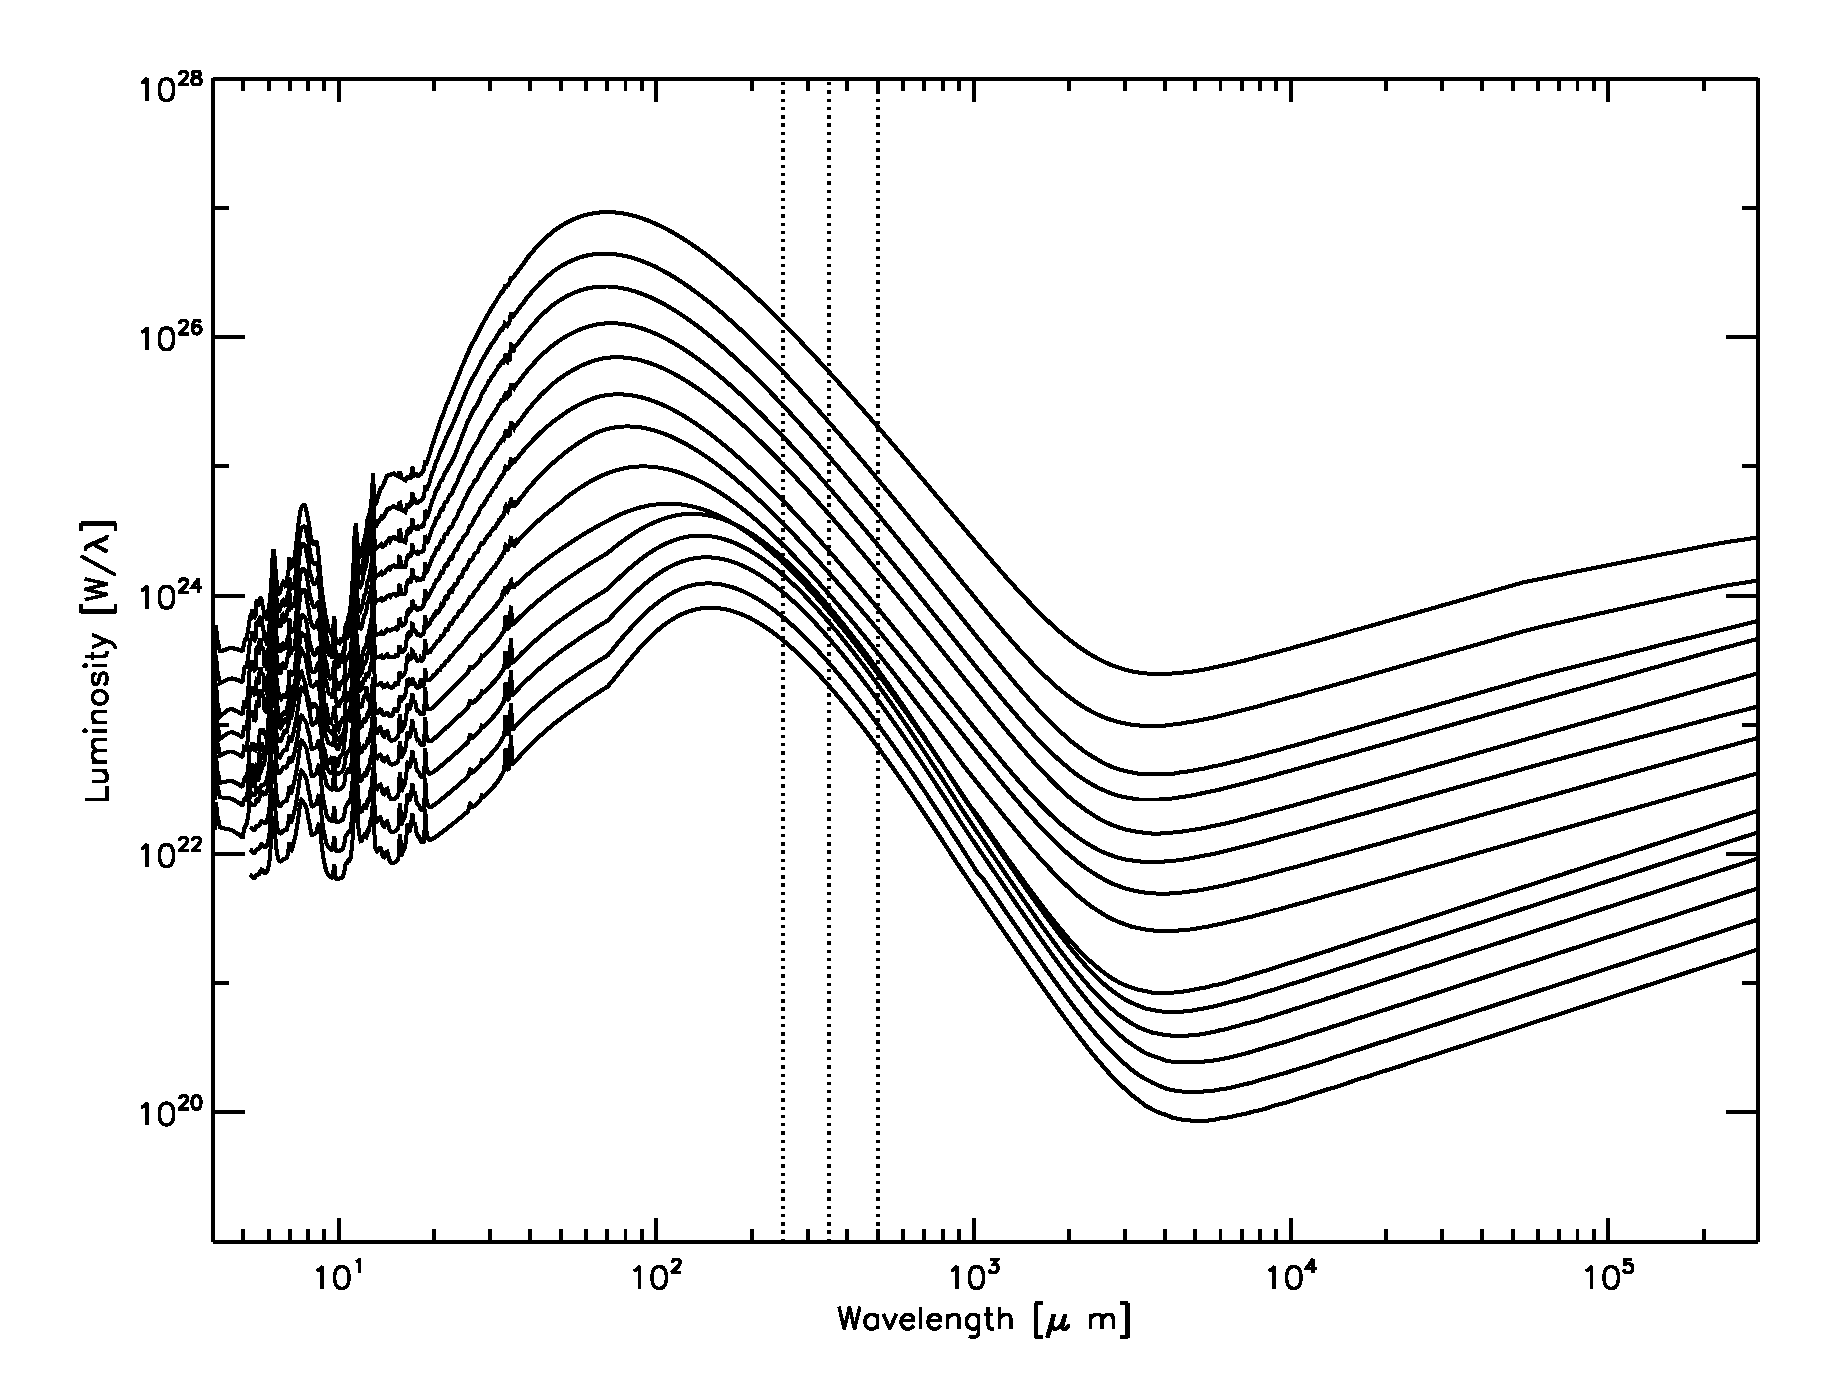
\includegraphics[width=\textwidth,trim=0.25in 0.25in 0.25in 0.25in,clip=true]{models.eps}
  \caption{SED Library consisting of LIRG and URLIRG templates ranging in far-infrared luminosity from $10^9$ to $10^13$ $L_{sun}$, taken from \citet{rieke09}. These templates are based on a mix of data from local galaxies and models of galaxies as modified blackbodies in the far-infrared regime, mixed with radio-loud tails seen on the far right of the models in the above plot. The transition between LIRG and ULIRG can be seen where the models seem to group through the FIR region. Currently, these models are used with their associated luminosities over the entire redshift range, however with color evolution we would see intrinsic luminosities increase with redshift without a corresponding temperature rise (these models will rise along the Luminosity axis with redshift).}
  \label{slib}
\end{figure*}

\begin{figure*}
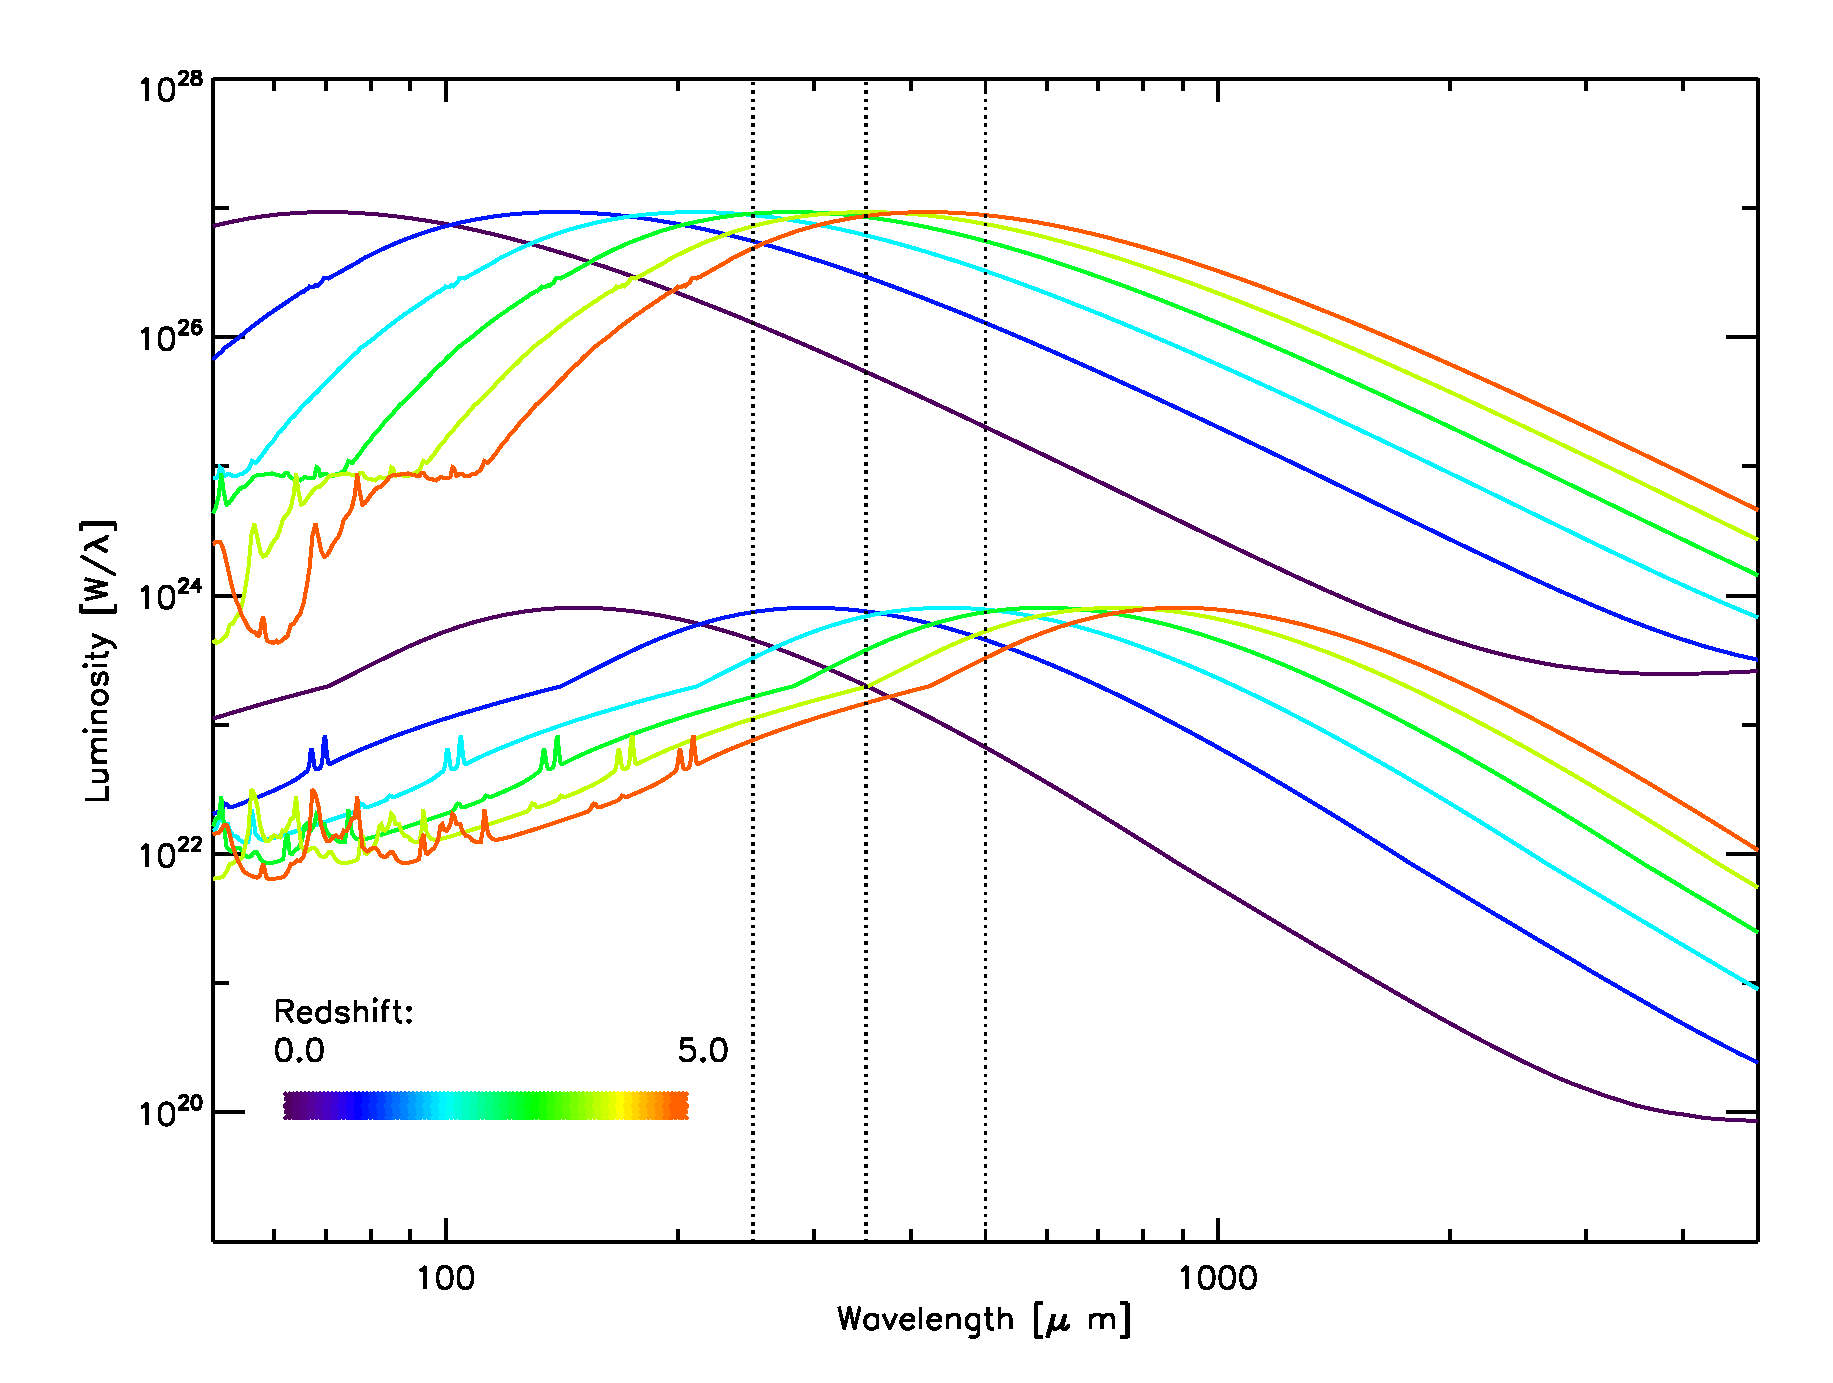
\includegraphics[width=\textwidth]{model_brightness.eps}
\caption{A visual of how the intensity and slope of the SED varies as a function of redshift. Here we see the brightest and faintest SED models from the \citet{rieke09} template library, redshifted between $z=0$ and $z=5$ in steps of $z=1$. We can see that intrinsic luminosity increases from low redshift, and slope rises from negative to positive with redshift. This helps to explain the overall trend we see when projecting the models into our color-color space.}
\label{mshift}
\end{figure*}

\begin{figure*}
  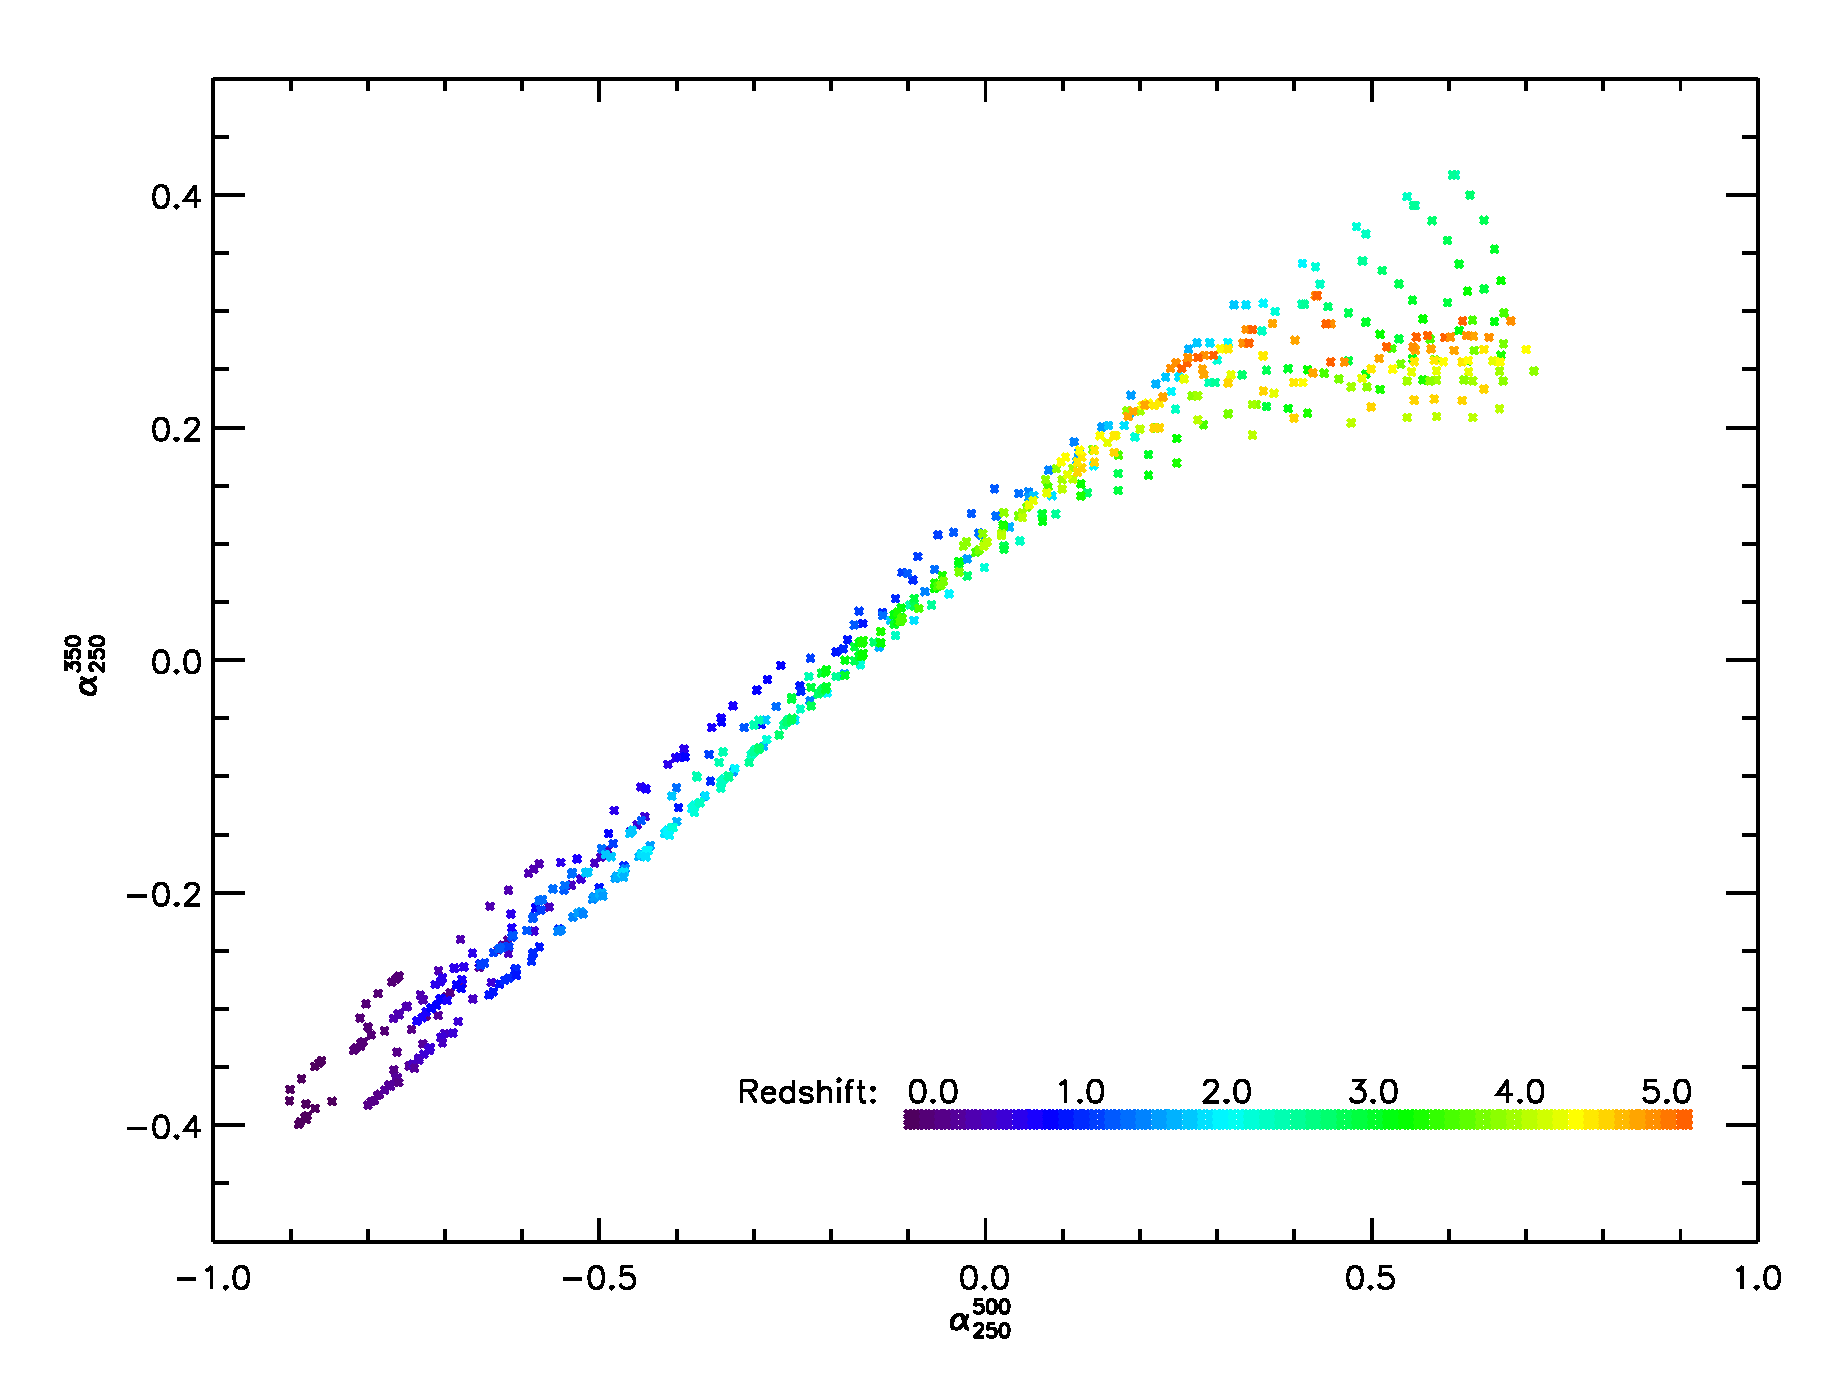
\includegraphics[width=\textwidth]{model_colors.eps}
  \caption{The spectral color pairs produced by the entire library of models for $0<z<5$, without added noise. Here we can see the general trend associated with redshift, however also a degeneracy between intrinsic luminosity and redshift along the trend line, as well as some natural dispersion due to natural variation in template form through the far-infrared region.}
  \label{slib_color}
\end{figure*}

\begin{figure*}
\centering
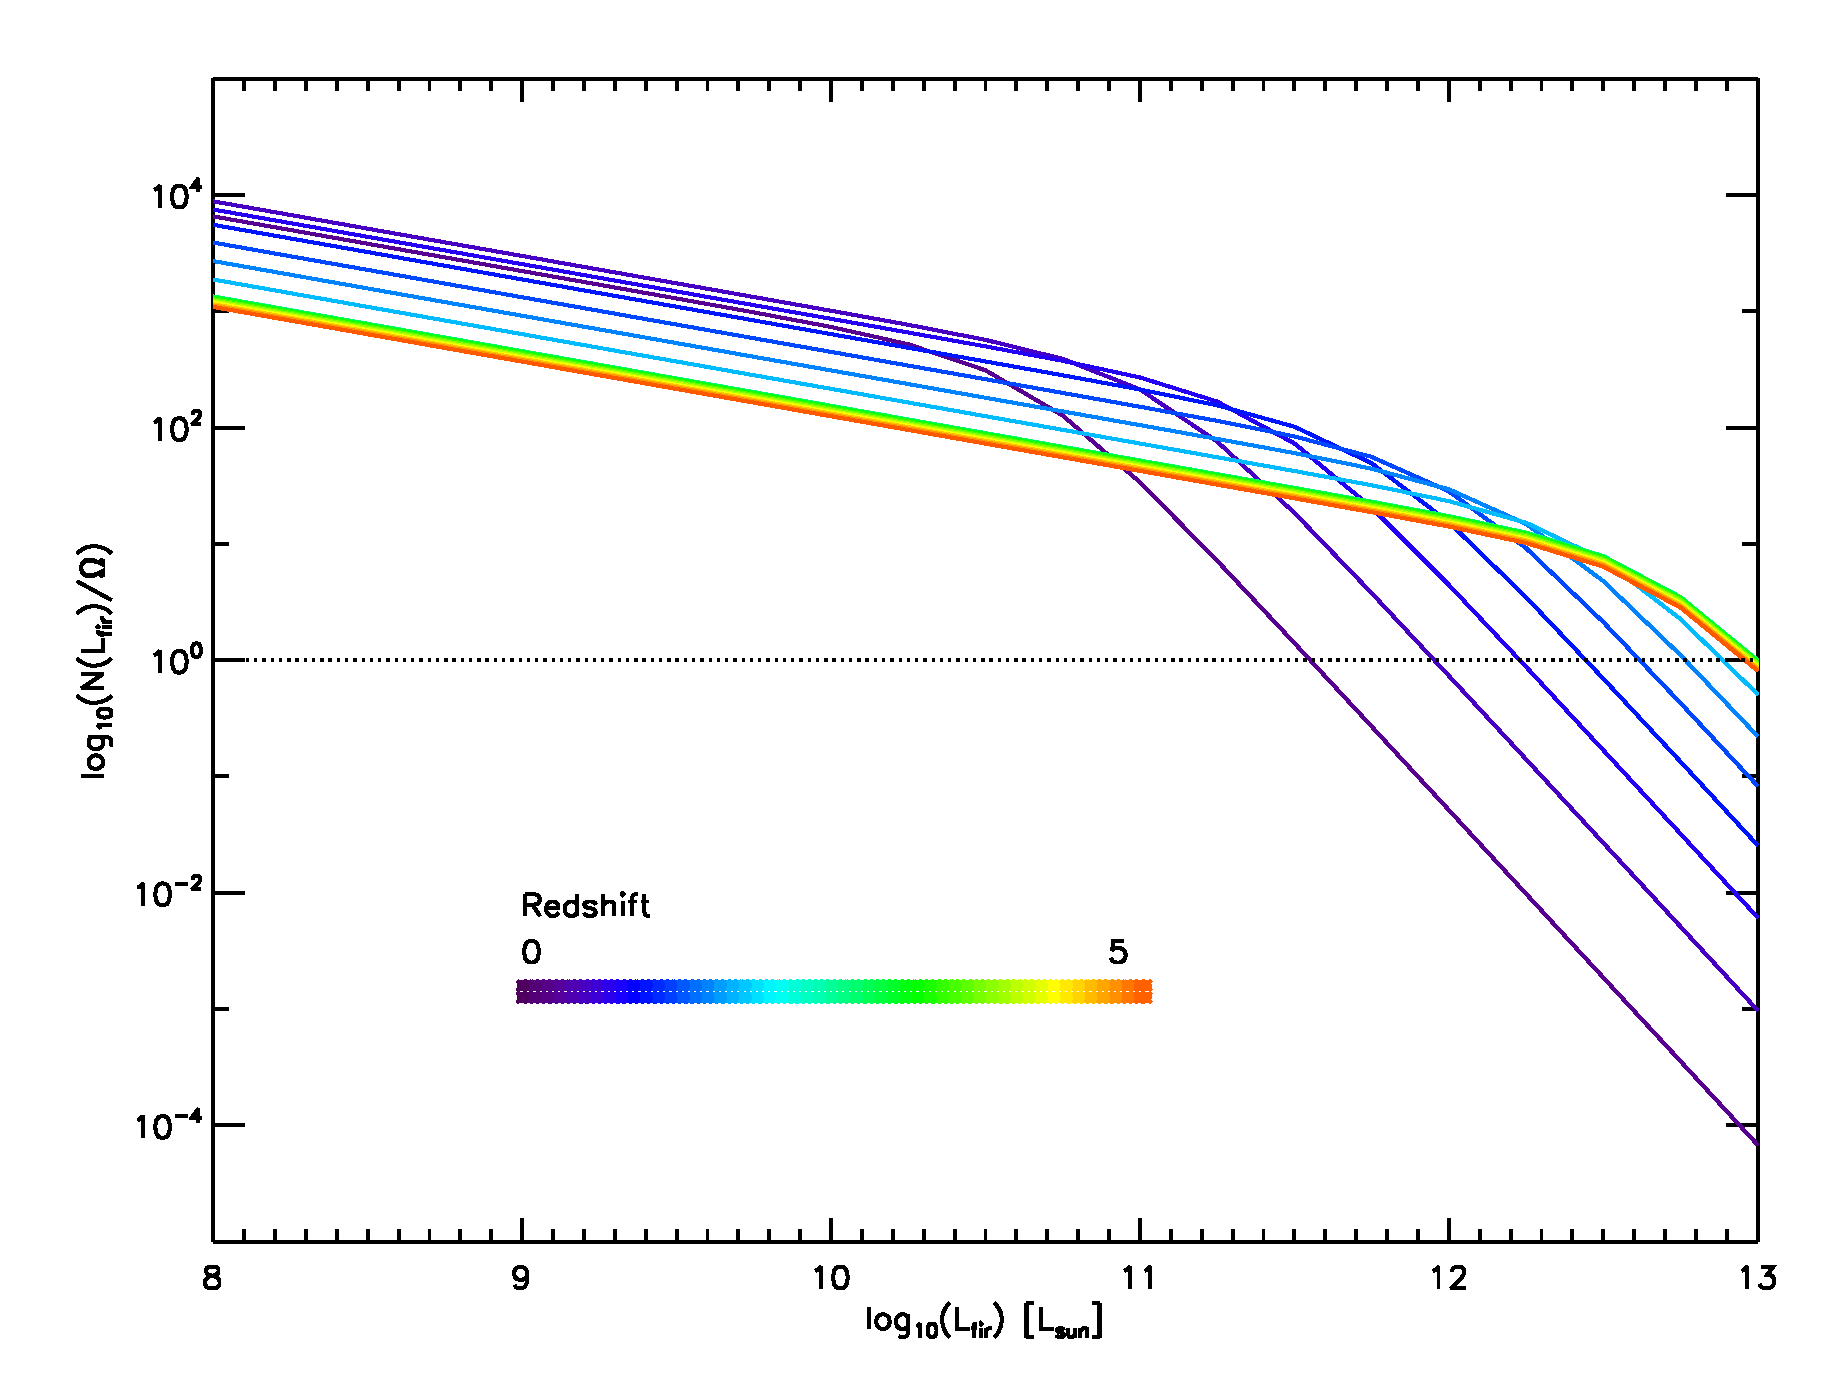
\includegraphics[width=\textwidth]{sim_lumfunct.eps}
\caption{Luminosity function from \citet{negrello13}, evolved with the parameter values fitted during a short sample simulation starting from the low-redshift \citet{Caputi07} values. Here we see evolution out to redshift of 2, and before that point positive evolution in characteristic luminosity and negative evolution in number density at this luminosity. The net product is to increase relative density of high luminosity galaxies such that they are more dominant in the sample at higher redshift; this combined with the relatively high magnitude limits of the samples we consider results in most of our sources being very bright and high redshift (see figure \ref{disp:res})}
\label{lf}
\end{figure*}

\begin{figure*}
  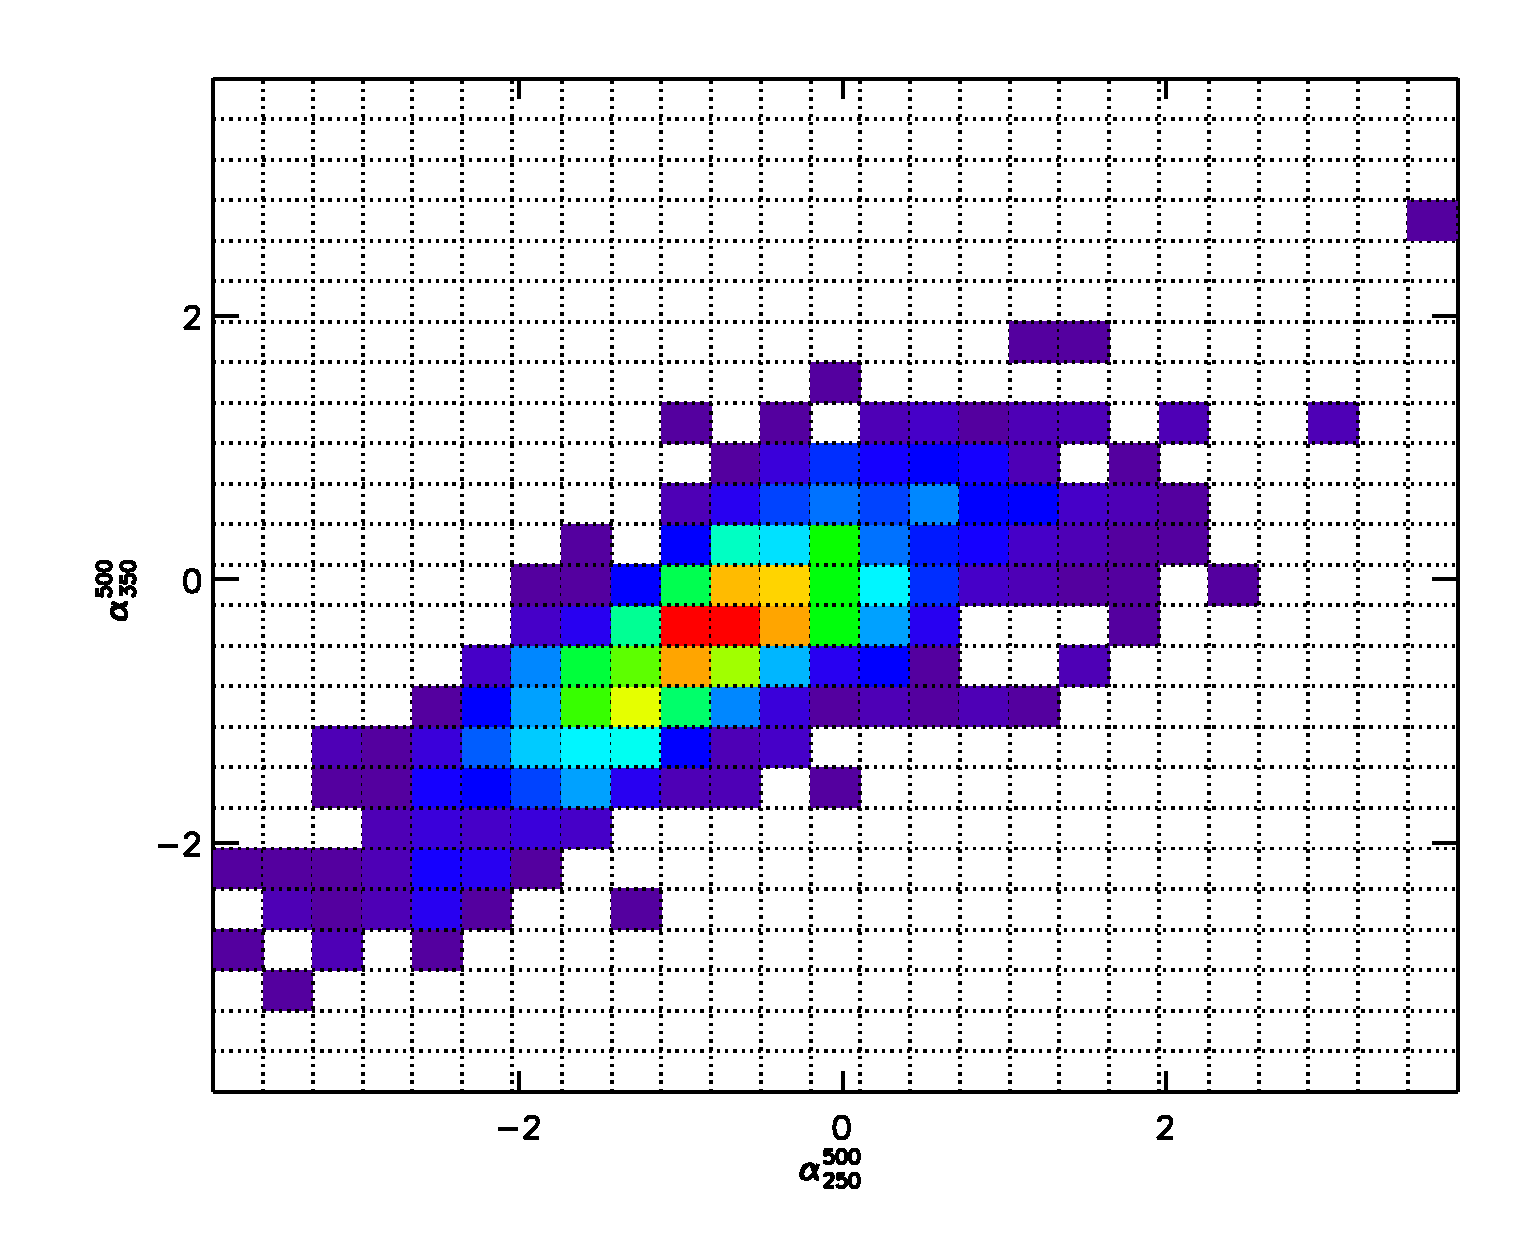
\includegraphics[width=\textwidth]{obs_color_hist.eps}
  \caption{An example of 2-D Color Histogram, created with the HerMES survey data \citep{HerMES}. This survey contains $\sim 10^3$ sources.}
  \label{fig:hist1}
\end{figure*}

\begin{figure*}
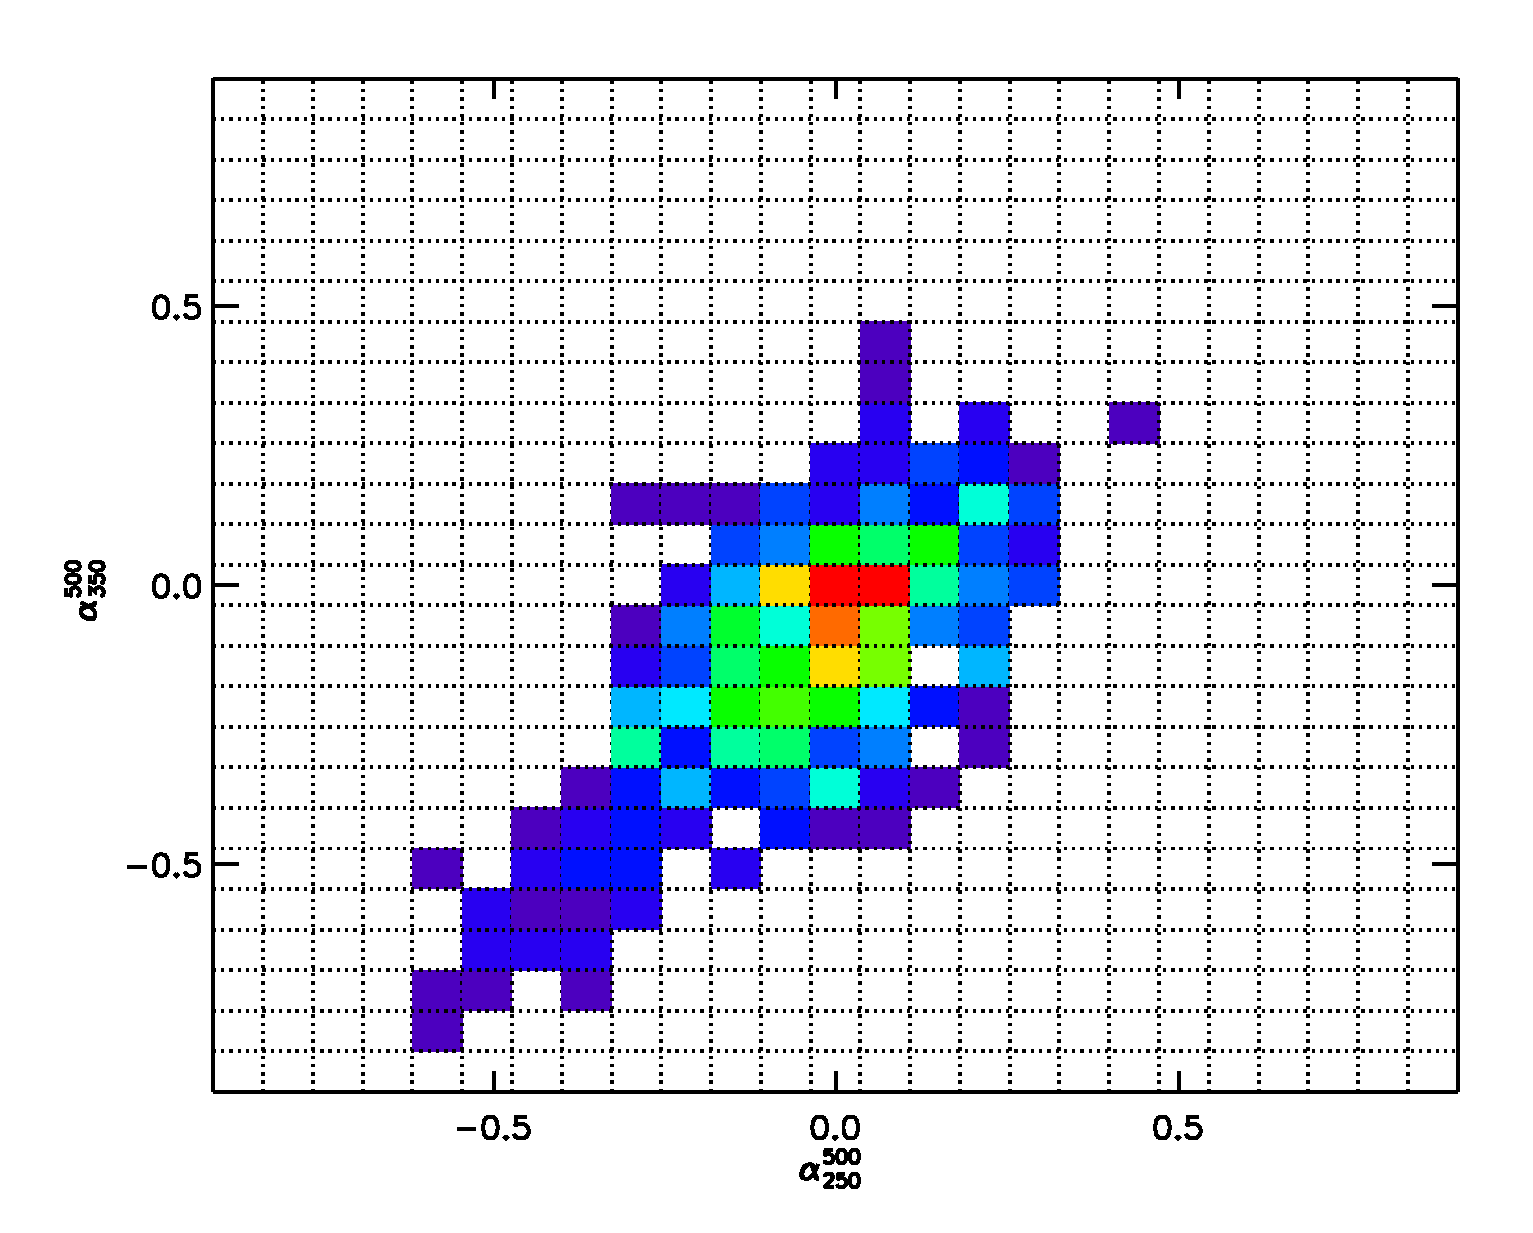
\includegraphics[width=\textwidth]{model_color_hist.eps}
\caption{An example of a simulated survey. This was created from a simulation with a very small number of iterations, and is meant to serve as an illustration as opposed to a realistic simulation. We do see a nice spread off of the zero noise model slope, and see that the simulation is at least heading in the right direction as compared to the observations.}
\label{simmed}
\end{figure*}

\begin{figure*}
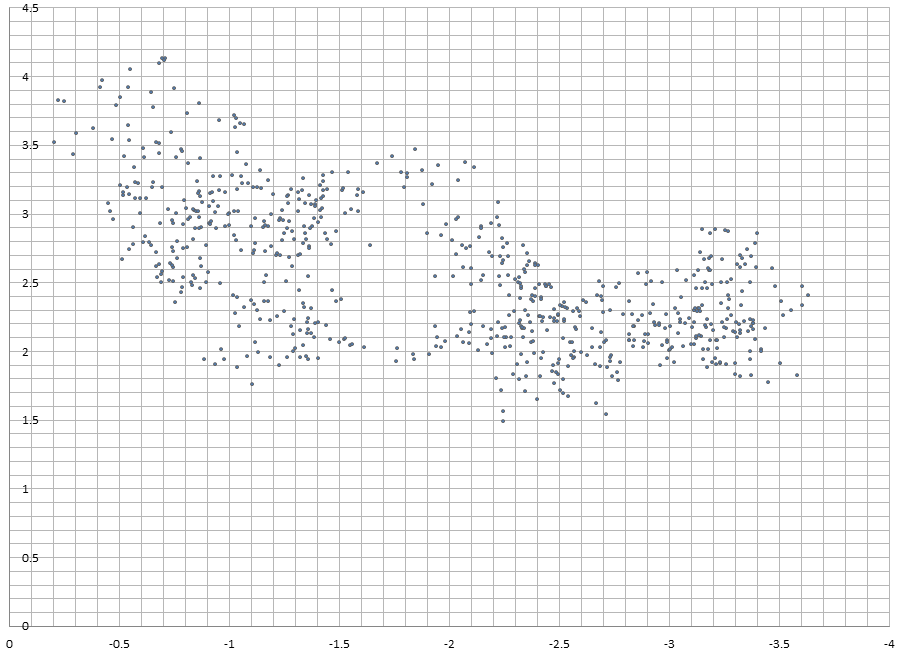
\includegraphics[width=\textwidth]{MCTest}
\caption{Example of parameter space exploration by the Monte Carlo algorithm, with p on the x axis and q on the y axis. What is most evident from this early demonstration is that there is definite clumping (indicative of a found minimum) but the Monte Carlo may be too hot, accepting guesses too often and moving too far from the minimum to proceed back quickly. Alternatively, the models could be partially inadequate, with different parts satisfying different aspects of observation and allowing multiple ``most likely'' peaks in our Monte Carlo. The above is only about 700 runs, so the space is inadequately sampled, however shows that the Monte Carlo is operating on the correct principles and finding minima.}
\label{fig:mc}
\end{figure*}

\begin{figure*}
  \centering
  \includegraphics[width=5 in]{initial.png}
  \caption{The IDL initial fitting window. At the top are the band parameters, below are the redshift and model parameters, and to the right are the luminosity function and cosmological parameters. The run simulation button creates fits files and runs the C++ executable, while the plot last run button reads the output.fits file in the current directory and produces the output seen in Figure \ref{disp:res}.}
  \label{disp:init}
\end{figure*}

\begin{figure*}
  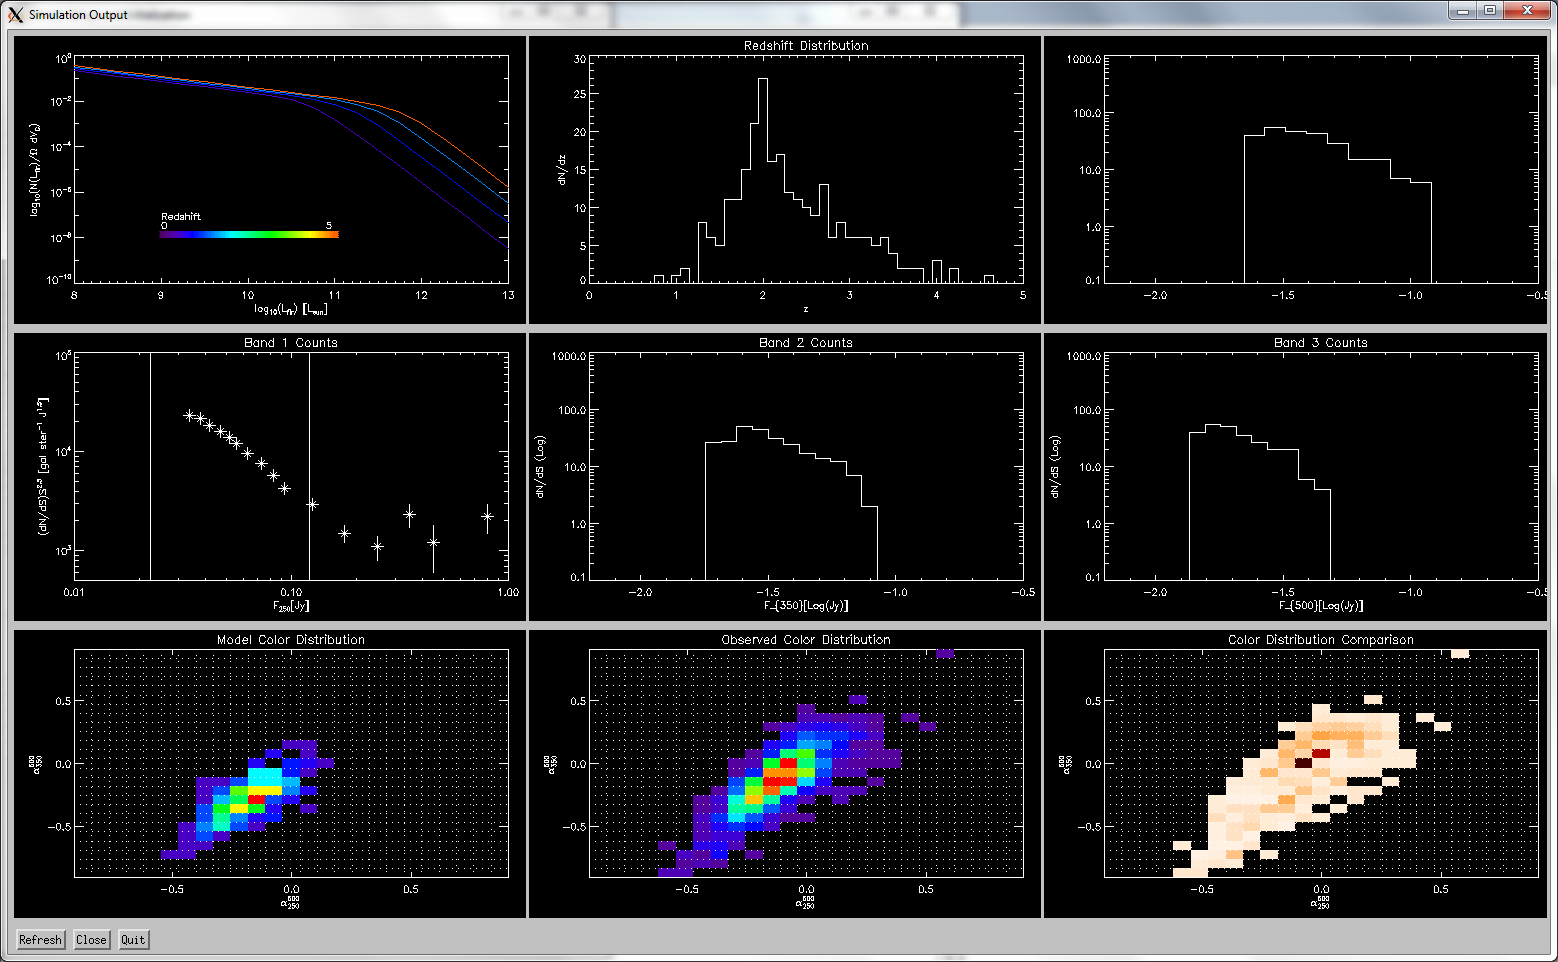
\includegraphics[width=\textwidth]{bestfit2.png}
  \caption{The IDL results display. The top row of the display (left to right) shows the luminosity function for the fitted parameters, as well as the resulting redshift distribution of simulated sources and a histogram of fluxes for the 250 $\mu m$ band. The second row shows more differential source counts, however evolution effects have not been removed in the second two panels, as they will in future version. The final row shows the model, observed, and comparison histograms from the simulation.}
  \label{disp:res}
\end{figure*}

\end{document}
